\documentclass[12pt,aspectratio=43]{beamer}

% 自訂字體的封包
\usepackage{fontspec}

% 導入圖形與表格的封包
\usepackage{graphicx}
\graphicspath{{./20251126_Meeting}}

\usepackage{booktabs}

% 排列多個子圖形的封包
\usepackage{subfigure} 

 % 提供進階數學環境與公式排版
\usepackage{mathtools, amsmath, amsfonts, amsthm, latexsym} 

%% 設定中文字體
\usepackage{xeCJK}
\setCJKmainfont[AutoFakeBold=3.5 , AutoFakeSlant=0.2]{標楷體}
\setmainfont{Times New Roman}
\XeTeXlinebreaklocale "zh"
\XeTeXlinebreakskip = 0pt plus 1pt

% 自訂字體顏色的封包
\usepackage{color} 

% 圖表自動編號的封包
\usepackage{caption} 

% 允許表格的一格能多列呈現的封包
\usepackage{multirow} 

% 可指定表格排版的封包
\usepackage{array}

% 翻轉表格的封包
\usepackage{lscape} 

% 序列標號
\usepackage{enumerate} 

%% 設定自動編號
\setbeamertemplate{caption}[numbered]

%% 自訂顏色
\definecolor{Myblue}{RGB}{57,108,144}
\definecolor{Default_Blue}{RGB}{52,51,171}

% (動畫)字會若隱若現的顯示
\beamersetuncovermixins{\opaqueness<1->{45}}{\opaqueness<1->{95}} 

% 設定中文的標籤
\renewcommand{\figurename}{圖} 
\renewcommand{\tablename}{表} 

% 排版形式 
\mode<presentation>{
\usetheme{Berlin}
% enumerate 及 item 的形狀
\setbeamertemplate{itemize items}[triangle]
% 調整外框形式的字體大小
\setbeamerfont{headline}{size=\scriptsize}
\setbeamerfont{footline}{size=\scriptsize}
% 取消右下方的跳轉工具列
\setbeamertemplate{navigation symbols}{} 
% 自定義2：清除外框下緣但僅出頁碼
\setbeamertemplate{footline}[page number] 
% 顏色主題
\usecolortheme{dove}
% 設定頁面邊界
\setbeamersize{text margin left=0.6cm, text margin right=0.6cm}
\special{papersize=\the\paperwidth,\the\paperheight}
\providecommand{\tabularnewline}{\\}
}

\title{Meeting 1126}
\author{黃丞暘}
\institute{國立東華大學應數統計所}
\date{November 26, 2025}

\begin{document}

% 封面
\begin{frame}
  \titlepage
\end{frame}

% 目錄
\begin{frame}{\textbf{Index}}
  \tableofcontents
\end{frame}

% 研究動機 
\section{Research motivation}

\begin{frame}{\textbf{Research motivation}}
\linespread{1.5}
  Semiconductor Manufacturing Process
  \begin{itemize}
    \item Unbox $y = \hat{f}(x)$
  \end{itemize}
  \begin{itemize}
    \item Timing to use SMOTE (deal with imbalanced data)
  \end{itemize}
  \begin{itemize}
    \item Fitting model
  \end{itemize}
\end{frame}

% 研究方法
\section{Research method}

\begin{frame}{\textbf{Research method}}
\linespread{1.5}
  \begin{itemize}[]
    \item Dimensionality reduction
      \begin{enumerate}[]
        \item PCA
      \end{enumerate}
    \item Clustering
      \begin{enumerate}[]
        \item KMeans
        \item AgglomerativeClustering(Hierarchical clustering)
      \end{enumerate}
    \item Model training(StandardScaler, SMOTE on training dataset)
      \begin{enumerate}
        \item LR, SVM, DT, RF, XGB
        \item ACC, FAR
      \end{enumerate}
  \end{itemize}
\end{frame}

% 結果
\section{Results}

\begin{frame}{\textbf{Results I}　{PCA + KMeans, 2 clusters}}
\linespread{0.9}

\begin{center}
	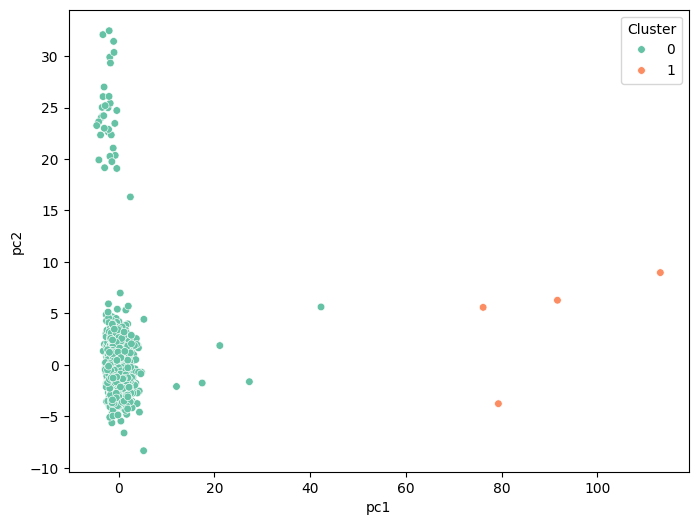
\includegraphics[scale=0.4]{PCA0.png}
\end{center}
\vspace{-0.1cm}
\small{$$
\begin{array}{c|cc}
\text{cluster} & 0 & 1 \\
\hline
y=0 & 1460 & 3 \\
y=1 & 103  & 1 \\
\end{array}
$$}

\end{frame}

\begin{frame}{\textbf{Results II}　{PCA + KMeans, 2 clusters}}
\linespread{0.9}

\begin{center}
\begin{minipage}{0.3\linewidth}
	\centering
	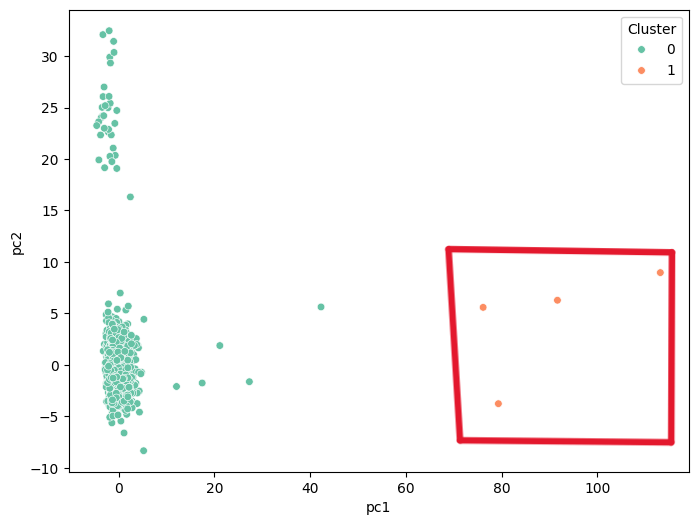
\includegraphics[width=\linewidth]{PCA0r1.png}
\end{minipage}
\hspace{0.3em}
\begin{minipage}{0.5\linewidth}
	\centering
	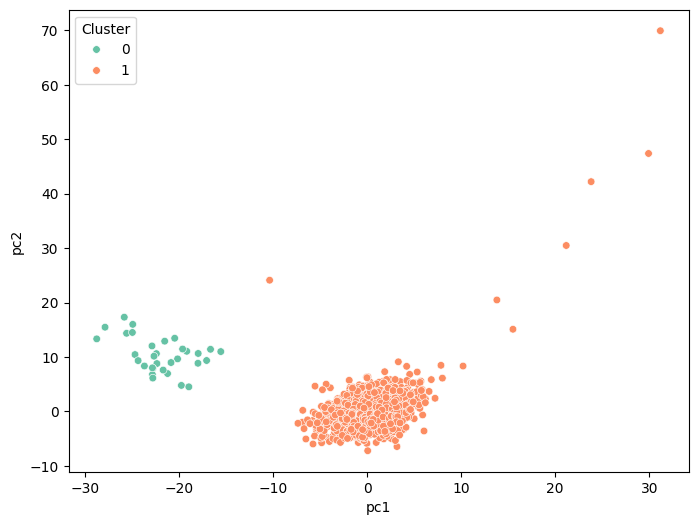
\includegraphics[width=\linewidth]{PCA01.png}
\end{minipage}
\end{center}

\small{$$
\begin{array}{c|cc}
\text{cluster} & 0 & 1 \\
\hline
y=0 & 1435 & 25 \\
y=1 & 96  & 7 \\
\end{array}
$$}

\end{frame}

\begin{frame}{\textbf{Results III}　{PCA + KMeans, 2 clusters}}
\linespread{0.9}

\begin{center}
\begin{minipage}{0.3\linewidth}
	\centering
	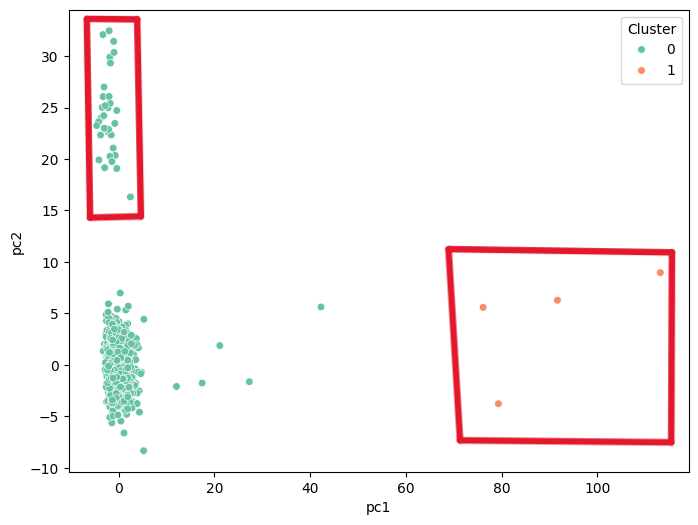
\includegraphics[width=\linewidth]{PCA0r2.png}
\end{minipage}
\hspace{0.3em}
\begin{minipage}{0.5\linewidth}
	\centering
	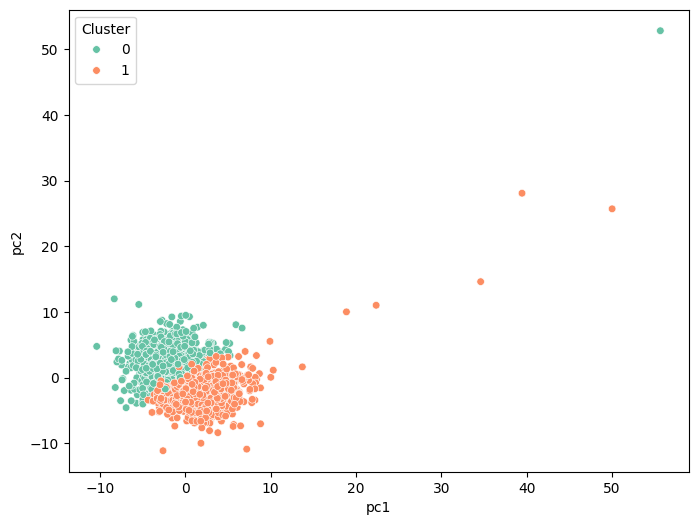
\includegraphics[width=\linewidth]{PCA02.png}
\end{minipage}
\end{center}

\small{$$
\begin{array}{c|cc}
\text{cluster} & 0 & 1 \\
\hline
y=0 & 669 & 765 \\
y=1 & 60  & 36 \\
\end{array}
$$}

\end{frame}

\begin{frame}{\textbf{Results III}　{Training in cluster 0}}
\linespread{0.9}
{\small
\begin{figure}[h]
\centering

%---------------------- 第一列 ----------------------
\begin{minipage}{0.28\linewidth}
\raggedright
{\small LR}
$$
\small
\begin{bmatrix}
122 & 12 \\
10  & 2
\end{bmatrix}
$$
\end{minipage}
\begin{minipage}{0.28\linewidth}
\raggedright
{\small SVM}
$$
\small
\begin{bmatrix}
133 & 1 \\
12  & 0
\end{bmatrix}
$$
\end{minipage}
\begin{minipage}{0.28\linewidth}
\raggedright
{\small DT}
$$
\small
\begin{bmatrix}
113 & 21 \\
8  & 4
\end{bmatrix}
$$
\end{minipage}

\vspace{0.5em}

%---------------------- 第二列 ----------------------
\begin{minipage}{0.28\linewidth}
\raggedright
{\small RF}
$$
\small
\begin{bmatrix}
134 & 0 \\
12  & 0
\end{bmatrix}
$$
\end{minipage}
\begin{minipage}{0.28\linewidth}
\raggedright
{\small XGB}
$$
\small
\begin{bmatrix}
130 & 4 \\
12  & 0
\end{bmatrix}
$$
\end{minipage}

\end{figure}
}

%---------------------- 第三列：Summary ----------------------
{\small
Summary
$$
\begin{array}{l|cc}
\text{model} & \text{ACC} & \text{FAR} \\
\hline
\text{LR} & 0.8493 & 0.0896 \\
\text{SVM} & 0.9110 & 0.0075 \\
\text{DT} & 0.8014 & 0.1567 \\
\text{RF} & 0.9178 & 0.0000 \\
\text{XGB} & 0.8904 & 0.0299 \\
\end{array}
$$
}

\end{frame}

\begin{frame}{\textbf{Results III}　{Training in cluster 1}}
\linespread{0.9}
{\small
\begin{figure}[h]
\centering

%---------------------- 第一列 ----------------------
\begin{minipage}{0.28\linewidth}
\raggedright
{\small LR}
$$
\small
\begin{bmatrix}
149 & 6 \\
5  & 2
\end{bmatrix}
$$
\end{minipage}
\begin{minipage}{0.28\linewidth}
\raggedright
{\small SVM}
$$
\small
\begin{bmatrix}
154 & 0 \\
7  & 0
\end{bmatrix}
$$
\end{minipage}
\begin{minipage}{0.28\linewidth}
\raggedright
{\small DT}
$$
\small
\begin{bmatrix}
141 & 13 \\
5  & 2
\end{bmatrix}
$$
\end{minipage}

\vspace{0.5em}

%---------------------- 第二列 ----------------------
\begin{minipage}{0.28\linewidth}
\raggedright
{\small RF}
$$
\small
\begin{bmatrix}
154 & 0 \\
7  & 0
\end{bmatrix}
$$
\end{minipage}
\begin{minipage}{0.28\linewidth}
\raggedright
{\small XGB}
$$
\small
\begin{bmatrix}
153 & 1 \\
7  & 0
\end{bmatrix}
$$
\end{minipage}

\end{figure}
}

%---------------------- 第三列：Summary ----------------------
{\small
Summary
$$
\begin{array}{l|cc}
\text{model} & \text{ACC} & \text{FAR} \\
\hline
\text{LR} & 0.9379 & 0.0325 \\
\text{SVM} & 0.9565 & 0.0000 \\
\text{DT} & 0.8882 & 0.0844\\
\text{RF} & 0.9565 & 0.0000 \\
\text{XGB} & 0.9503 & 0.0065 \\
\end{array}
$$
}

\end{frame}

\begin{frame}{\textbf{Results IV}　{PCA + KMeans, 2 clusters}}
\linespread{0.9}

\begin{center}
\begin{minipage}{0.3\linewidth}
	\centering
	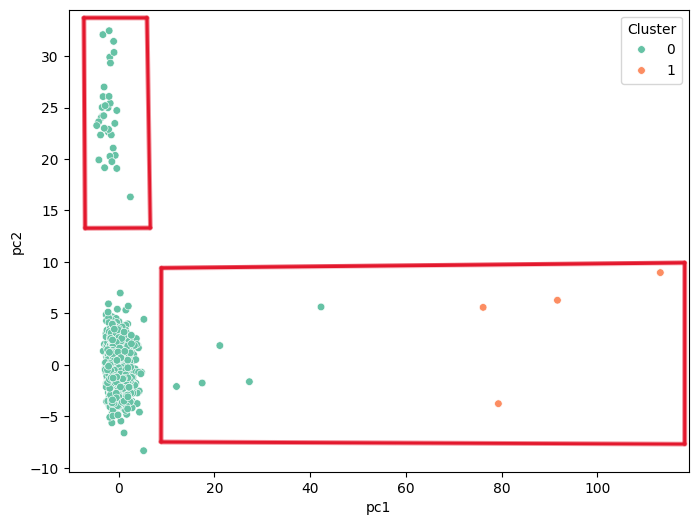
\includegraphics[width=\linewidth]{PCA0r3.png}
\end{minipage}
\hspace{0.3em}
\begin{minipage}{0.5\linewidth}
	\centering
	
\includegraphics[width=\linewidth]{PCA1.png}
\end{minipage}
\end{center}

\small{$$
\begin{array}{c|cc}
\text{cluster} & 0 & 1 \\
\hline
y=0 & 660 & 770 \\
y=1 & 58  & 37 \\
\end{array}
$$}

\end{frame}

\begin{frame}{\textbf{Results IV}　{Training in cluster 0}}
\linespread{0.9}
{\small
\begin{figure}[h]
\centering

%---------------------- 第一列 ----------------------
\begin{minipage}{0.28\linewidth}
\raggedright
{\small LR}
$$
\small
\begin{bmatrix}
114 & 18 \\
6  & 6
\end{bmatrix}
$$
\end{minipage}
\begin{minipage}{0.28\linewidth}
\raggedright
{\small SVM}
$$
\small
\begin{bmatrix}
131 & 1 \\
12  & 0
\end{bmatrix}
$$
\end{minipage}
\begin{minipage}{0.28\linewidth}
\raggedright
{\small DT}
$$
\small
\begin{bmatrix}
117 & 15 \\
10  & 2
\end{bmatrix}
$$
\end{minipage}

\vspace{0.5em}

%---------------------- 第二列 ----------------------
\begin{minipage}{0.28\linewidth}
\raggedright
{\small RF}
$$
\small
\begin{bmatrix}
132 & 0 \\
12  & 0
\end{bmatrix}
$$
\end{minipage}
\begin{minipage}{0.28\linewidth}
\raggedright
{\small XGB}
$$
\small
\begin{bmatrix}
129 & 3 \\
12  & 0
\end{bmatrix}
$$
\end{minipage}

\end{figure}
}

%---------------------- 第三列：Summary ----------------------
{\small
Summary
$$
\begin{array}{l|cc}
\text{model} & \text{ACC} & \text{FAR} \\
\hline
\text{LR} & 0.8333 & 0.1364 \\
\text{SVM} & 0.9097 & 0.0076 \\
\text{DT} & 0.8264 & 0.1136\\
\text{RF} & 0.9167 & 0.0000 \\
\text{XGB} & 0.8958 & 0.0227 \\
\end{array}
$$
}

\end{frame}

\begin{frame}{\textbf{Results IV}　{Training in cluster 1}}
\linespread{0.9}
{\small
\begin{figure}[h]
\centering

%---------------------- 第一列 ----------------------
\begin{minipage}{0.28\linewidth}
\raggedright
{\small LR}
$$
\small
\begin{bmatrix}
141 & 14 \\
6  & 1
\end{bmatrix}
$$
\end{minipage}
\begin{minipage}{0.28\linewidth}
\raggedright
{\small SVM}
$$
\small
\begin{bmatrix}
155 & 0 \\
7  & 0
\end{bmatrix}
$$
\end{minipage}
\begin{minipage}{0.28\linewidth}
\raggedright
{\small DT}
$$
\small
\begin{bmatrix}
136 & 19 \\
6  & 1
\end{bmatrix}
$$
\end{minipage}

\vspace{0.5em}

%---------------------- 第二列 ----------------------
\begin{minipage}{0.28\linewidth}
\raggedright
{\small RF}
$$
\small
\begin{bmatrix}
155 & 0 \\
7  & 0
\end{bmatrix}
$$
\end{minipage}
\begin{minipage}{0.28\linewidth}
\raggedright
{\small XGB}
$$
\small
\begin{bmatrix}
155 & 0 \\
7  & 0
\end{bmatrix}
$$
\end{minipage}

\end{figure}
}

%---------------------- 第三列：Summary ----------------------
{\small
Summary
$$
\begin{array}{l|cc}
\text{model} & \text{ACC} & \text{FAR} \\
\hline
\text{LR} & 0.8765 & 0.0903 \\
\text{SVM} & 0.9568 & 0.0000 \\
\text{DT} & 0.8457 & 0.1226\\
\text{RF} & 0.9568 & 0.0000 \\
\text{XGB} & 0.9568 & 0.000 \\
\end{array}
$$
}

\end{frame}


% --- 結束 ---
\section*{結束}

\begin{frame}[plain] % 產生無外框的頁面
	\begin{center}
		{\Huge The End}
		\bigskip\bigskip 

		{\LARGE Questions  \&  Comments}
	\end{center}
\end{frame}
\end{document}ㄒ
